% !TeX program = xelatex
% !TeX encoding = UTF-8
%
% 学生通常只需要修改本文件、chapters/ 下的章节文件和 references.bib。
% swutthesis.cls 是学校版式实现文件，一般不需要在写作过程中修改。
\documentclass{swutthesis}

% ============================================================================
% 1. 参考文献数据库
% ============================================================================
\addbibresource{references.bib}

% ============================================================================
% 2. 论文基本信息（请替换花括号中的示例内容）
% ============================================================================
% 完整题目：同时用于封面、页眉、PDF 书签和文档元数据。
% 封面会按题目框宽度自动换行；不要复制 Word 标题中的手动换行。
\thesistitle{主标题示例：本科毕业论文规范写作示例}

% 仅当封面显示文本需要与完整题目不同时，才使用下方覆盖命令。
% \coverthesistitle{封面专用标题}

% 可选副标题：显示为封面题目区的第三行；没有副标题时删除或注释此行。
\thesissubtitle{副标题示例：以某高校为例}

\studentname{张三}
\studentid{2026000000}
\college{信息工程学院}
\major{计算机科学与技术}
% 一位教师直接填写姓名；两位教师用英文逗号分隔，封面会自动分成两行。
% 两字姓名自动空开一个汉字宽度，三字姓名保持紧排。
\supervisor{李老师}
% \supervisor{李明,王小华}
\coverdate{二〇二六年六月}

% 诚信承诺书与版权使用授权声明的日期；如需打印后手写，可将三项留空。
\commitmentdate{2026}{6}{20}
\authorizationdate{2026}{6}{20}

% 可选电子签名：同一张签名图用于两处时使用 \authorsignature。
% 若两处签名不同，改用 \commitmentsignature 和
% \authorizationsignature 分别设置。请勿把真实签名提交到公共仓库。
% \authorsignature{assets/signature.png}
% \commitmentsignature{assets/commitment-signature.png}
% \authorizationsignature{assets/authorization-signature.png}

% ============================================================================
% 3. 文档开始
% ============================================================================
\begin{document}

% 封面、诚信承诺书与版权使用授权声明（声明紧接封面，为 PDF 第 2 页）
\maketitle
\makecopyrightstatements

% ----------------------------------------------------------------------------
% 中文摘要
% ----------------------------------------------------------------------------
\begin{cnabstract}
摘要应是一篇能够独立阅读的内容概括。在不依赖正文、图表和注释的
情况下，依次交代毕业设计（论文）的研究目的、研究对象或核心问题、
采用的方法与实施过程、获得的主要结果、形成的结论，以及具有价值
的创新或实践贡献。开头可用一至两句话说明研究要解决的问题及其
意义，随后说明数据、材料、技术路线或分析方法，再用准确的定量或
定性表述给出最重要的发现，最后概括结论、适用范围和必要的限制。
若研究包含多项结果，应按照重要程度组织，而不是照搬正文目录逐项
罗列。摘要不宜写成长篇背景介绍，不引用参考文献，不使用图表、公式
和脚注，也不写“本文将在”等尚未完成的计划性表述。语言应客观、
凝练、完整，避免空泛评价、宣传性措辞和无法验证的绝对化结论。
中文摘要一般以三百至五百字为宜，并与正文结论及英文摘要保持一致。
完成全文后，应再次核对摘要中的研究对象、样本数量、关键数据和主要
结论，确保读者仅阅读摘要即可理解论文研究了什么、怎样开展研究、
得到了什么结果，以及这些结果具有什么理论意义或实践价值。
\cnkeywords{研究目的；研究方法；研究结果；主要结论}
\end{cnabstract}

% ----------------------------------------------------------------------------
% 英文摘要
% ----------------------------------------------------------------------------
\begin{enabstract}
An abstract should provide a self-contained account of the graduation project
or thesis. Without requiring the reader to consult the main text, figures, or
notes, it should state the research objective, the object or central question,
the methods and procedures, the principal results, the conclusions, and any
meaningful theoretical or practical contribution. The opening sentences may
identify the problem and explain why it deserves investigation. The following
sentences should describe the data, materials, technical route, experiment, or
analytical method used in the study. The most important findings should then
be reported with precise quantitative or qualitative evidence, followed by a
concise conclusion and, where necessary, the scope and limitations of the
result. If several findings are presented, they should be ordered by
importance instead of repeating the chapter sequence. The abstract should not
become an extended literature review, cite references, or contain figures,
tables, formulas, and footnotes. It should also avoid promises such as “this
study will” after the research has been completed. Objective and verifiable
language is preferred to promotional claims or unsupported superlatives. An
English abstract of approximately 200 to 300 words is recommended and should
correspond to the Chinese abstract in research content and conclusions. After
the full thesis has been revised, the author should verify the research object,
sample size, key data, and conclusions stated in both abstracts so that a
reader can understand what was studied, how the work was conducted, what was
found, and why the findings matter.
\enkeywords{research objective; research method; research result; main conclusion}
\end{enabstract}

% 目录及图表清单均由章节、图题和表题自动生成。
\swuttableofcontents
\listoffiguresandtables

% ============================================================================
% 4. 正文
% ============================================================================
\mainmatter
% 第一章：按照本模板的实际使用顺序介绍最常用的 LaTeX 操作。
\chapter{模板快速上手}

\section{本章目的与阅读方式}

本章用于帮助第一次接触 LaTeX 的学生完成模板配置和基本内容修改，
不属于毕业设计（论文）的正式研究内容。建议在开始写作前完整阅读
一遍，并对照源文件实际操作；掌握基本使用方法后，正式提交论文时
可以删除本章及其在 \texttt{main.tex} 中对应的
\verb|% 第一章：按照本模板的实际使用顺序介绍最常用的 LaTeX 操作。
\chapter{模板快速上手}

\section{本章目的与阅读方式}

本章用于帮助第一次接触 LaTeX 的学生完成模板配置和基本内容修改，
不属于毕业设计（论文）的正式研究内容。建议在开始写作前完整阅读
一遍，并对照源文件实际操作；掌握基本使用方法后，正式提交论文时
可以删除本章及其在 \texttt{main.tex} 中对应的
\verb|% 第一章：按照本模板的实际使用顺序介绍最常用的 LaTeX 操作。
\chapter{模板快速上手}

\section{本章目的与阅读方式}

本章用于帮助第一次接触 LaTeX 的学生完成模板配置和基本内容修改，
不属于毕业设计（论文）的正式研究内容。建议在开始写作前完整阅读
一遍，并对照源文件实际操作；掌握基本使用方法后，正式提交论文时
可以删除本章及其在 \texttt{main.tex} 中对应的
\verb|\include{chapters/latex-quickstart}| 命令。

LaTeX 的基本工作方式是“在源文件中描述文档结构，再由编译器生成
PDF”。学生只需使用本章介绍的少量命令组织标题、段落、图表和文献，
模板会自动处理学校要求的字体、字号、行距、编号、目录和页码。

\section{从哪里开始修改}

完成论文写作主要涉及三个位置：
\begin{enumerate}
  \item \texttt{main.tex}：填写封面信息、中英文摘要、致谢和附录，
        并安排各章的先后顺序；
  \item \texttt{chapters/}：保存正文各章，每一章对应一个
        \texttt{.tex} 文件；
  \item \texttt{references.bib}：保存参考文献数据。
\end{enumerate}

\texttt{swutthesis.cls} 负责字体、字号、行距、页眉页脚和目录等版式，
正常写作时不修改该文件。模板会自动完成排版，不需要在正文中重复
设置宋体、黑体、字号、行距或页码。

\section{填写论文基本信息}

\texttt{main.tex} 开头集中放置封面信息。花括号中的示例文字应替换为
论文的实际信息：

% 封面命令与 main.tex 保持一致，便于直接对照修改。
\begin{lstlisting}[language={[LaTeX]TeX}]
\thesistitle{论文完整题目}
\coverthesistitle{封面题目第一行\\封面题目第二行}
\thesissubtitle{副标题}

\studentname{姓名}
\studentid{学号}
\college{学院名称}
\major{专业名称}
\supervisor{指导教师}
\coverdate{二〇二六年六月}

\commitmentdate{2026}{6}{20}
\authorizationdate{2026}{6}{20}
\end{lstlisting}

\verb|\thesistitle| 中填写不换行的完整题目，用于页眉和 PDF 信息。
封面需要换成两行时，在 \verb|\coverthesistitle| 中使用一次
\verb|\\|。没有副标题时，删除或注释 \verb|\thesissubtitle| 所在行。
\verb|\commitmentdate{年}{月}{日}| 和
\verb|\authorizationdate{年}{月}{日}| 分别填写诚信承诺书与版权使用
授权声明的日期。如需在打印后手写日期，可将对应命令写为
\verb|\commitmentdate{}{}{}| 或 \verb|\authorizationdate{}{}{}|。

中文摘要写在 \texttt{cnabstract} 环境中，关键词写入
\verb|\cnkeywords{...}|；英文摘要写在 \texttt{enabstract} 环境中，
关键词写入 \verb|\enkeywords{...}|。直接替换模板中的示例内容即可，
摘要标题、缩进、行距和关键词样式均会自动生成。

\section{建立正文各章}

正文文件统一放在 \texttt{chapters/} 目录中。例如，新建
\texttt{chapters/method.tex} 后，可按以下结构开始写作：

\begin{lstlisting}[language={[LaTeX]TeX},float=htbp]
\chapter{研究方法}

\section{总体方案}
这里填写正文。

\subsection{数据来源}
这里填写正文。

\subsubsection{样本筛选}
这里填写正文。
\end{lstlisting}

四个标题命令在 PDF 中依次显示为“第一章”“1.1”“1.1.1”和“（1）”
等层级。标题文字中不输入编号，目录和编号由模板自动生成。

新建的章节文件还需要在 \texttt{main.tex} 正文区域加入：

\begin{lstlisting}[language={[LaTeX]TeX}]
\include{chapters/method}
\end{lstlisting}

\verb|\include| 的排列顺序就是最终的章节顺序。文件名末尾的
\texttt{.tex} 不写入命令。

\section{输入正文和分段}

正文直接输入在相应标题下方。两段文字之间保留一个空行，模板会自动
设置首行缩进和段落行距：

\begin{lstlisting}[language={[LaTeX]TeX}]
这是第一个自然段。源文件中的普通换行不会开始新段落，
PDF 会根据页面宽度自动断行。

这是第二个自然段。两个自然段之间保留一个空行。
\end{lstlisting}

普通正文不使用 \verb|\\| 换段，也不使用连续空格或空行调整位置。
百分号 \verb|%| 后面的内容只作为源文件注释，不会显示在 PDF 中。
正文中需要显示百分号、下划线或连接符号时，分别写成
\verb|\%|、\verb|\_| 和 \verb|\&|。

\section{插入图片、表格和公式}

图片文件放入 \texttt{assets/} 目录，再复制以下代码并替换文件名和
图题：

\begin{lstlisting}[language={[LaTeX]TeX},float=htbp]
\begin{figure}[htbp]
  \centering
  \includegraphics[width=0.72\textwidth]{assets/图片文件名.png}
  \caption{图片标题}
  \label{fig:图片标识}
\end{figure}

如图~\ref{fig:图片标识} 所示，……
\end{lstlisting}

\verb|\label| 中的标识只在源文件中使用，每个标识应保持唯一。
正文通过 \verb|\ref| 引用图号，图片移动后编号会自动更新。

表格和公式的完整标准写法已放在
\texttt{chapters/academic-writing.tex} 中。实际写作时复制其中一个
完整示例，再替换表题、数据或公式内容即可。表格使用
\texttt{table} 和 \texttt{swuttable}，独立编号的公式使用
\texttt{equation}；编号均由模板自动生成。

\section{引用参考文献}

\texttt{references.bib} 已包含图书、期刊论文、学位论文、标准和网络
资料等示例。新增文献时，复制类型最接近的一条记录，修改作者、题名、
年份等字段，并设置一个不重复的引用键。例如，数据库中已有引用键
\texttt{wu2010film}，正文引用方式为：

\begin{lstlisting}[language={[LaTeX]TeX}]
薄膜生长过程具有明显的阶段性特征\cite{wu2010film}。
\end{lstlisting}

文献序号和文末参考文献表会自动生成。正式论文中删除
\texttt{main.tex} 里的 \verb|\nocite{*}| 后，参考文献表只列出正文
实际引用的记录。

按照学校 Word 模板中的写作要求，正式论文参考文献一般不少于 20 篇，
其中外文文献不少于 5 篇，书籍不多于 5 部，教材不列入参考文献。
文末列出的每条文献都应在正文相应位置实际引用，并核对作者、题名、
年份、页码、网址和访问日期等信息。

\section{编译并查看结果}

如果系统已经安装并配置好 \texttt{latexmk}，可在项目根目录运行：

\begin{lstlisting}[language=bash]
latexmk main.tex
\end{lstlisting}

编译完成后查看 \texttt{main.pdf}。修改标题、图表、公式或参考文献后，
仍使用同一条命令重新编译；\texttt{latexmk} 会自动完成目录、编号、
交叉引用和参考文献所需的多轮处理。

部分 MiKTeX Basic 环境没有预装可直接使用的 \texttt{latexmk}。此时
不需要更换模板，可依次执行下面四条命令：

\begin{lstlisting}[language=bash]
xelatex main.tex
biber main
xelatex main.tex
xelatex main.tex
\end{lstlisting}

第一轮 XeLaTeX 生成辅助文件，Biber 处理参考文献，后两轮 XeLaTeX
更新目录、页码和交叉引用。使用 TeXstudio 时，也可以把构建流程配置
为“XeLaTeX → Biber → XeLaTeX → XeLaTeX”。

写作过程中只维护论文内容，不手工输入章节编号、图表编号、页码或
目录点线，也不通过空格和换行模拟版式。模板中的示例可以直接复制，
替换内容后重新编译即可。

\section{进入论文正文示例}

从下一章开始，文档按照“绪论—研究设计与实施—研究结果与规范表达—
讨论与论文组织—总结与展望”的顺序，演示本科毕业设计（论文）的
基本结构，并给出各部分可以参考的写作内容。后续文字用于说明每一
部分应解决的问题，而不是要求学生原样保留；正式写作时应结合本专业
特点、研究任务和指导教师意见替换为自己的论文内容。
| 命令。

LaTeX 的基本工作方式是“在源文件中描述文档结构，再由编译器生成
PDF”。学生只需使用本章介绍的少量命令组织标题、段落、图表和文献，
模板会自动处理学校要求的字体、字号、行距、编号、目录和页码。

\section{从哪里开始修改}

完成论文写作主要涉及三个位置：
\begin{enumerate}
  \item \texttt{main.tex}：填写封面信息、中英文摘要、致谢和附录，
        并安排各章的先后顺序；
  \item \texttt{chapters/}：保存正文各章，每一章对应一个
        \texttt{.tex} 文件；
  \item \texttt{references.bib}：保存参考文献数据。
\end{enumerate}

\texttt{swutthesis.cls} 负责字体、字号、行距、页眉页脚和目录等版式，
正常写作时不修改该文件。模板会自动完成排版，不需要在正文中重复
设置宋体、黑体、字号、行距或页码。

\section{填写论文基本信息}

\texttt{main.tex} 开头集中放置封面信息。花括号中的示例文字应替换为
论文的实际信息：

% 封面命令与 main.tex 保持一致，便于直接对照修改。
\begin{lstlisting}[language={[LaTeX]TeX}]
\thesistitle{论文完整题目}
\coverthesistitle{封面题目第一行\\封面题目第二行}
\thesissubtitle{副标题}

\studentname{姓名}
\studentid{学号}
\college{学院名称}
\major{专业名称}
\supervisor{指导教师}
\coverdate{二〇二六年六月}

\commitmentdate{2026}{6}{20}
\authorizationdate{2026}{6}{20}
\end{lstlisting}

\verb|\thesistitle| 中填写不换行的完整题目，用于页眉和 PDF 信息。
封面需要换成两行时，在 \verb|\coverthesistitle| 中使用一次
\verb|\\|。没有副标题时，删除或注释 \verb|\thesissubtitle| 所在行。
\verb|\commitmentdate{年}{月}{日}| 和
\verb|\authorizationdate{年}{月}{日}| 分别填写诚信承诺书与版权使用
授权声明的日期。如需在打印后手写日期，可将对应命令写为
\verb|\commitmentdate{}{}{}| 或 \verb|\authorizationdate{}{}{}|。

中文摘要写在 \texttt{cnabstract} 环境中，关键词写入
\verb|\cnkeywords{...}|；英文摘要写在 \texttt{enabstract} 环境中，
关键词写入 \verb|\enkeywords{...}|。直接替换模板中的示例内容即可，
摘要标题、缩进、行距和关键词样式均会自动生成。

\section{建立正文各章}

正文文件统一放在 \texttt{chapters/} 目录中。例如，新建
\texttt{chapters/method.tex} 后，可按以下结构开始写作：

\begin{lstlisting}[language={[LaTeX]TeX},float=htbp]
\chapter{研究方法}

\section{总体方案}
这里填写正文。

\subsection{数据来源}
这里填写正文。

\subsubsection{样本筛选}
这里填写正文。
\end{lstlisting}

四个标题命令在 PDF 中依次显示为“第一章”“1.1”“1.1.1”和“（1）”
等层级。标题文字中不输入编号，目录和编号由模板自动生成。

新建的章节文件还需要在 \texttt{main.tex} 正文区域加入：

\begin{lstlisting}[language={[LaTeX]TeX}]
\include{chapters/method}
\end{lstlisting}

\verb|\include| 的排列顺序就是最终的章节顺序。文件名末尾的
\texttt{.tex} 不写入命令。

\section{输入正文和分段}

正文直接输入在相应标题下方。两段文字之间保留一个空行，模板会自动
设置首行缩进和段落行距：

\begin{lstlisting}[language={[LaTeX]TeX}]
这是第一个自然段。源文件中的普通换行不会开始新段落，
PDF 会根据页面宽度自动断行。

这是第二个自然段。两个自然段之间保留一个空行。
\end{lstlisting}

普通正文不使用 \verb|\\| 换段，也不使用连续空格或空行调整位置。
百分号 \verb|%| 后面的内容只作为源文件注释，不会显示在 PDF 中。
正文中需要显示百分号、下划线或连接符号时，分别写成
\verb|\%|、\verb|\_| 和 \verb|\&|。

\section{插入图片、表格和公式}

图片文件放入 \texttt{assets/} 目录，再复制以下代码并替换文件名和
图题：

\begin{lstlisting}[language={[LaTeX]TeX},float=htbp]
\begin{figure}[htbp]
  \centering
  \includegraphics[width=0.72\textwidth]{assets/图片文件名.png}
  \caption{图片标题}
  \label{fig:图片标识}
\end{figure}

如图~\ref{fig:图片标识} 所示，……
\end{lstlisting}

\verb|\label| 中的标识只在源文件中使用，每个标识应保持唯一。
正文通过 \verb|\ref| 引用图号，图片移动后编号会自动更新。

表格和公式的完整标准写法已放在
\texttt{chapters/academic-writing.tex} 中。实际写作时复制其中一个
完整示例，再替换表题、数据或公式内容即可。表格使用
\texttt{table} 和 \texttt{swuttable}，独立编号的公式使用
\texttt{equation}；编号均由模板自动生成。

\section{引用参考文献}

\texttt{references.bib} 已包含图书、期刊论文、学位论文、标准和网络
资料等示例。新增文献时，复制类型最接近的一条记录，修改作者、题名、
年份等字段，并设置一个不重复的引用键。例如，数据库中已有引用键
\texttt{wu2010film}，正文引用方式为：

\begin{lstlisting}[language={[LaTeX]TeX}]
薄膜生长过程具有明显的阶段性特征\cite{wu2010film}。
\end{lstlisting}

文献序号和文末参考文献表会自动生成。正式论文中删除
\texttt{main.tex} 里的 \verb|\nocite{*}| 后，参考文献表只列出正文
实际引用的记录。

按照学校 Word 模板中的写作要求，正式论文参考文献一般不少于 20 篇，
其中外文文献不少于 5 篇，书籍不多于 5 部，教材不列入参考文献。
文末列出的每条文献都应在正文相应位置实际引用，并核对作者、题名、
年份、页码、网址和访问日期等信息。

\section{编译并查看结果}

如果系统已经安装并配置好 \texttt{latexmk}，可在项目根目录运行：

\begin{lstlisting}[language=bash]
latexmk main.tex
\end{lstlisting}

编译完成后查看 \texttt{main.pdf}。修改标题、图表、公式或参考文献后，
仍使用同一条命令重新编译；\texttt{latexmk} 会自动完成目录、编号、
交叉引用和参考文献所需的多轮处理。

部分 MiKTeX Basic 环境没有预装可直接使用的 \texttt{latexmk}。此时
不需要更换模板，可依次执行下面四条命令：

\begin{lstlisting}[language=bash]
xelatex main.tex
biber main
xelatex main.tex
xelatex main.tex
\end{lstlisting}

第一轮 XeLaTeX 生成辅助文件，Biber 处理参考文献，后两轮 XeLaTeX
更新目录、页码和交叉引用。使用 TeXstudio 时，也可以把构建流程配置
为“XeLaTeX → Biber → XeLaTeX → XeLaTeX”。

写作过程中只维护论文内容，不手工输入章节编号、图表编号、页码或
目录点线，也不通过空格和换行模拟版式。模板中的示例可以直接复制，
替换内容后重新编译即可。

\section{进入论文正文示例}

从下一章开始，文档按照“绪论—研究设计与实施—研究结果与规范表达—
讨论与论文组织—总结与展望”的顺序，演示本科毕业设计（论文）的
基本结构，并给出各部分可以参考的写作内容。后续文字用于说明每一
部分应解决的问题，而不是要求学生原样保留；正式写作时应结合本专业
特点、研究任务和指导教师意见替换为自己的论文内容。
| 命令。

LaTeX 的基本工作方式是“在源文件中描述文档结构，再由编译器生成
PDF”。学生只需使用本章介绍的少量命令组织标题、段落、图表和文献，
模板会自动处理学校要求的字体、字号、行距、编号、目录和页码。

\section{从哪里开始修改}

完成论文写作主要涉及三个位置：
\begin{enumerate}
  \item \texttt{main.tex}：填写封面信息、中英文摘要、致谢和附录，
        并安排各章的先后顺序；
  \item \texttt{chapters/}：保存正文各章，每一章对应一个
        \texttt{.tex} 文件；
  \item \texttt{references.bib}：保存参考文献数据。
\end{enumerate}

\texttt{swutthesis.cls} 负责字体、字号、行距、页眉页脚和目录等版式，
正常写作时不修改该文件。模板会自动完成排版，不需要在正文中重复
设置宋体、黑体、字号、行距或页码。

\section{填写论文基本信息}

\texttt{main.tex} 开头集中放置封面信息。花括号中的示例文字应替换为
论文的实际信息：

% 封面命令与 main.tex 保持一致，便于直接对照修改。
\begin{lstlisting}[language={[LaTeX]TeX}]
\thesistitle{论文完整题目}
\coverthesistitle{封面题目第一行\\封面题目第二行}
\thesissubtitle{副标题}

\studentname{姓名}
\studentid{学号}
\college{学院名称}
\major{专业名称}
\supervisor{指导教师}
\coverdate{二〇二六年六月}

\commitmentdate{2026}{6}{20}
\authorizationdate{2026}{6}{20}
\end{lstlisting}

\verb|\thesistitle| 中填写不换行的完整题目，用于页眉和 PDF 信息。
封面需要换成两行时，在 \verb|\coverthesistitle| 中使用一次
\verb|\\|。没有副标题时，删除或注释 \verb|\thesissubtitle| 所在行。
\verb|\commitmentdate{年}{月}{日}| 和
\verb|\authorizationdate{年}{月}{日}| 分别填写诚信承诺书与版权使用
授权声明的日期。如需在打印后手写日期，可将对应命令写为
\verb|\commitmentdate{}{}{}| 或 \verb|\authorizationdate{}{}{}|。

中文摘要写在 \texttt{cnabstract} 环境中，关键词写入
\verb|\cnkeywords{...}|；英文摘要写在 \texttt{enabstract} 环境中，
关键词写入 \verb|\enkeywords{...}|。直接替换模板中的示例内容即可，
摘要标题、缩进、行距和关键词样式均会自动生成。

\section{建立正文各章}

正文文件统一放在 \texttt{chapters/} 目录中。例如，新建
\texttt{chapters/method.tex} 后，可按以下结构开始写作：

\begin{lstlisting}[language={[LaTeX]TeX},float=htbp]
\chapter{研究方法}

\section{总体方案}
这里填写正文。

\subsection{数据来源}
这里填写正文。

\subsubsection{样本筛选}
这里填写正文。
\end{lstlisting}

四个标题命令在 PDF 中依次显示为“第一章”“1.1”“1.1.1”和“（1）”
等层级。标题文字中不输入编号，目录和编号由模板自动生成。

新建的章节文件还需要在 \texttt{main.tex} 正文区域加入：

\begin{lstlisting}[language={[LaTeX]TeX}]
\include{chapters/method}
\end{lstlisting}

\verb|\include| 的排列顺序就是最终的章节顺序。文件名末尾的
\texttt{.tex} 不写入命令。

\section{输入正文和分段}

正文直接输入在相应标题下方。两段文字之间保留一个空行，模板会自动
设置首行缩进和段落行距：

\begin{lstlisting}[language={[LaTeX]TeX}]
这是第一个自然段。源文件中的普通换行不会开始新段落，
PDF 会根据页面宽度自动断行。

这是第二个自然段。两个自然段之间保留一个空行。
\end{lstlisting}

普通正文不使用 \verb|\\| 换段，也不使用连续空格或空行调整位置。
百分号 \verb|%| 后面的内容只作为源文件注释，不会显示在 PDF 中。
正文中需要显示百分号、下划线或连接符号时，分别写成
\verb|\%|、\verb|\_| 和 \verb|\&|。

\section{插入图片、表格和公式}

图片文件放入 \texttt{assets/} 目录，再复制以下代码并替换文件名和
图题：

\begin{lstlisting}[language={[LaTeX]TeX},float=htbp]
\begin{figure}[htbp]
  \centering
  \includegraphics[width=0.72\textwidth]{assets/图片文件名.png}
  \caption{图片标题}
  \label{fig:图片标识}
\end{figure}

如图~\ref{fig:图片标识} 所示，……
\end{lstlisting}

\verb|\label| 中的标识只在源文件中使用，每个标识应保持唯一。
正文通过 \verb|\ref| 引用图号，图片移动后编号会自动更新。

表格和公式的完整标准写法已放在
\texttt{chapters/academic-writing.tex} 中。实际写作时复制其中一个
完整示例，再替换表题、数据或公式内容即可。表格使用
\texttt{table} 和 \texttt{swuttable}，独立编号的公式使用
\texttt{equation}；编号均由模板自动生成。

\section{引用参考文献}

\texttt{references.bib} 已包含图书、期刊论文、学位论文、标准和网络
资料等示例。新增文献时，复制类型最接近的一条记录，修改作者、题名、
年份等字段，并设置一个不重复的引用键。例如，数据库中已有引用键
\texttt{wu2010film}，正文引用方式为：

\begin{lstlisting}[language={[LaTeX]TeX}]
薄膜生长过程具有明显的阶段性特征\cite{wu2010film}。
\end{lstlisting}

文献序号和文末参考文献表会自动生成。正式论文中删除
\texttt{main.tex} 里的 \verb|\nocite{*}| 后，参考文献表只列出正文
实际引用的记录。

按照学校 Word 模板中的写作要求，正式论文参考文献一般不少于 20 篇，
其中外文文献不少于 5 篇，书籍不多于 5 部，教材不列入参考文献。
文末列出的每条文献都应在正文相应位置实际引用，并核对作者、题名、
年份、页码、网址和访问日期等信息。

\section{编译并查看结果}

如果系统已经安装并配置好 \texttt{latexmk}，可在项目根目录运行：

\begin{lstlisting}[language=bash]
latexmk main.tex
\end{lstlisting}

编译完成后查看 \texttt{main.pdf}。修改标题、图表、公式或参考文献后，
仍使用同一条命令重新编译；\texttt{latexmk} 会自动完成目录、编号、
交叉引用和参考文献所需的多轮处理。

部分 MiKTeX Basic 环境没有预装可直接使用的 \texttt{latexmk}。此时
不需要更换模板，可依次执行下面四条命令：

\begin{lstlisting}[language=bash]
xelatex main.tex
biber main
xelatex main.tex
xelatex main.tex
\end{lstlisting}

第一轮 XeLaTeX 生成辅助文件，Biber 处理参考文献，后两轮 XeLaTeX
更新目录、页码和交叉引用。使用 TeXstudio 时，也可以把构建流程配置
为“XeLaTeX → Biber → XeLaTeX → XeLaTeX”。

写作过程中只维护论文内容，不手工输入章节编号、图表编号、页码或
目录点线，也不通过空格和换行模拟版式。模板中的示例可以直接复制，
替换内容后重新编译即可。

\section{进入论文正文示例}

从下一章开始，文档按照“绪论—研究设计与实施—研究结果与规范表达—
讨论与论文组织—总结与展望”的顺序，演示本科毕业设计（论文）的
基本结构，并给出各部分可以参考的写作内容。后续文字用于说明每一
部分应解决的问题，而不是要求学生原样保留；正式写作时应结合本专业
特点、研究任务和指导教师意见替换为自己的论文内容。

% 第二章示例：说明绪论各部分应回答的问题。
% 正式写作时应结合实际课题替换内容，文件名不影响章节编号。
\chapter{绪论}

\section{研究背景和意义}

绪论用于说明研究从何而来、为什么值得开展，以及论文准备解决什么
问题。研究背景应从所属技术领域、行业需求或理论问题逐步收束到具体
课题，避免堆砌与研究目标关系不大的宏观材料。研究意义可以分别说明
理论价值和实践价值，但应建立在真实问题和已有研究基础上，不宜使用
空泛口号或夸大性表述。

对于毕业设计类课题，还应交代应用场景、设计需求、主要约束和预期
成果；对于实证研究类课题，则应说明研究对象、关键现象和需要验证的
问题。背景、意义和后文研究目标之间应形成清楚的逻辑关系。

\section{国内外研究现状}

研究现状不是参考文献的逐篇摘要，而是围绕研究问题对已有成果进行
分类、比较和评价。作者可按照理论观点、研究方法、技术路线、应用
场景或时间发展过程组织文献，说明不同研究之间的联系、差异和不足。
引用他人观点、数据或方法时，应在正文相应位置标注文献来源
\cite{liu1988vortex,wu2010film,sui2015edm}。

本节结尾通常需要在文献分析基础上归纳尚未解决的问题，说明本文的
切入点。评价已有研究时应保持客观，既不能只罗列优点，也不能在缺少
证据的情况下笼统声称“国内研究较少”或“现有方法均存在缺陷”。

\section{研究目标与主要内容}

研究目标应与题目、研究问题和最终结论保持一致，并尽量使用可以检验
或评价的表述。主要内容用于说明为实现目标将完成哪些相互关联的工作，
而不是简单重复章节名称。一般可以从以下方面组织：

\begin{enumerate}
  \item 明确研究对象、问题边界、需求条件和评价指标；
  \item 说明采用的理论、模型、技术方案、实验方法或调查方法；
  \item 完成数据获取、系统实现、实验验证或案例分析；
  \item 对结果进行比较和解释，归纳结论、创新点与适用范围。
\end{enumerate}

若论文包含创新点，应准确说明创新发生在研究对象、方法、数据、
技术实现还是应用场景，避免把常规工作包装为创新。

\section{论文组织结构}

论文组织结构应简要说明各章承担的任务以及章与章之间的逻辑关系。
正式论文通常从绪论开始，随后依次展开理论基础或相关技术、研究设计
与实施、结果分析与讨论，最后给出总结与展望。不同专业可以根据课题
类型调整章节名称和顺序。

当前示例的第一章是模板使用教程，正式提交前可以删除。从本章开始，
后续章节依次演示研究设计、结果表达、讨论和总结等常见内容。组织
结构说明应随最终目录同步修改，不应保留与实际章节不一致的占位文字。

% 第二章示例：说明模板自动处理的页面与文字结构。
\chapter{模板结构与自动化处理}

\section{页面结构}

文档类统一管理论文的页面结构和各组成部分。学生只需在章节文件中
组织内容，不需要在正文中重复调用页面设置命令。

\section{页眉页脚与页码}

页眉内容根据论文题目自动生成，页码则按照前置部分、正文和后置部分
自动连续编排。学生无需在章节文件中手工插入页眉、页脚或页码。

\section{分页控制}

封面、声明、摘要、目录、正文章节和后置部分由模板自动建立分页关系。
图、表和代码块放不下时将整体转入下一页，后续段落不会越过这些内容
提前排版，从而保持源文件与最终论文的阅读顺序一致。

\section{中西文内容处理}

模板根据正文、标题、图表、公式和程序代码等内容类型自动选择相应的
中西文字体及段落样式。学生直接输入自然段即可，版式会随内容类型
自动应用。

% 第四章示例：说明结果写作，并展示脚注、公式、图表和程序代码。
\chapter{研究结果与规范表达}

\section{研究结果的组织}

研究结果部分应直接回应研究问题，并按照重要程度或分析逻辑组织
材料。作者需要先说明观察到的事实、数据或系统表现，再通过比较、
统计检验、案例证据或性能指标揭示其特征。正文不应逐项复述图表中的
全部数字，而应指出最值得关注的变化、差异、趋势和异常情况。

结果与讨论可以分章书写，也可以根据专业习惯合并。分章书写时，本章
主要呈现“发现了什么”，下一章重点解释“为什么出现这些结果”以及
“结果意味着什么”。无论采用哪种结构，都应区分客观结果与作者解释，
并确保每项结论都有相应证据支持。

\section{书写规范}

\subsection{使用语言}

原则上，毕业设计（论文）应采用国家语言文字工作委员会正式公布的
简化汉字书写。

\subsection{名词术语}

毕业设计（论文）中采用的术语、符号和代号必须全文统一，并符合相关
规范要求。

\subsubsection{科学技术名词}

科学技术名词应尽量采用全国科学技术名词审定委员会公布的规范词，
或国家相关标准中规定的名称。尚未统一规定或叫法有争议的名词术语，
可采用本学科惯用的名称。

\subsubsection{外文缩写和外国人名}

使用具有特定含义的术语、新名词或外文缩写时，首次出现应在圆括号
内注明含义或原文。外国人名一般可采用英文原名，广为人知的人名可按
通行标准译法书写。

\subsubsection{计量单位}

计量单位应符合国家标准 GB 3100～3102—93。非物理量的单位，如件、
台、人和元等，可使用汉字与符号构成组合单位，例如件/台、元/km。
单位名称应全文统一，不应混用中英文名称。

\subsection{数字和标点符号}

标点符号应符合《标点符号用法》（GB/T 15834—2011）。涉及测量和
统计的数据一般使用阿拉伯数字，在普通叙述中则应根据语言习惯合理
选择数字形式。

\section{注释与公式}

\subsection{注释}

正文中有个别名词或情况需要解释时，可以采用脚注。脚注序号以页为
单位，每页从 1 开始编号，正文中的编号使用上标；注释应置于注释
符号出现的同一页，不得隔页。\footnote{脚注可用于补充不宜在正文
展开、但有助于读者理解的说明。}

\subsection{公式}

数学公式用于准确表达变量之间的关系，重要公式应在正文中加以解释
和引用。二项式展开可写为
% equation 会自动按章编号；label 用于正文中的交叉引用。
\begin{equation}
  (1+x)^n
  = 1 + \frac{nx}{1!}
  + \frac{n(n-1)x^2}{2!} + \cdots .
  \label{eq:binomial}
\end{equation}

傅里叶级数可表示为
\begin{equation}
  f(x)=a_0+\sum_{n=1}^{\infty}
  \left(a_n\cos\frac{n\pi x}{L}
  +b_n\sin\frac{n\pi x}{L}\right).
  \label{eq:fourier}
\end{equation}

长公式不能在一行排完时，原则上应在等号或运算符处换行，并使运算符
位于续行行首。需要解释变量时，可在公式后使用“式中：$a_n$ 为余弦
项系数，$b_n$ 为正弦项系数”的形式说明。

\section{图表表达}

图表标题应简洁、精炼并具有自明性。图表应在正文首次提及之后给出，
并与相邻文字形成清晰、连贯的论证关系。

\subsection{图}

插图应保持背景清晰，横纵坐标的变量名、单位和刻度应完整。
图~\ref{fig:distribution} 给出了统计分布示例。

% 插图：先在正文中提及，再放置 figure；caption 在 label 之前。
\begin{figure}[htbp]
  \centering
  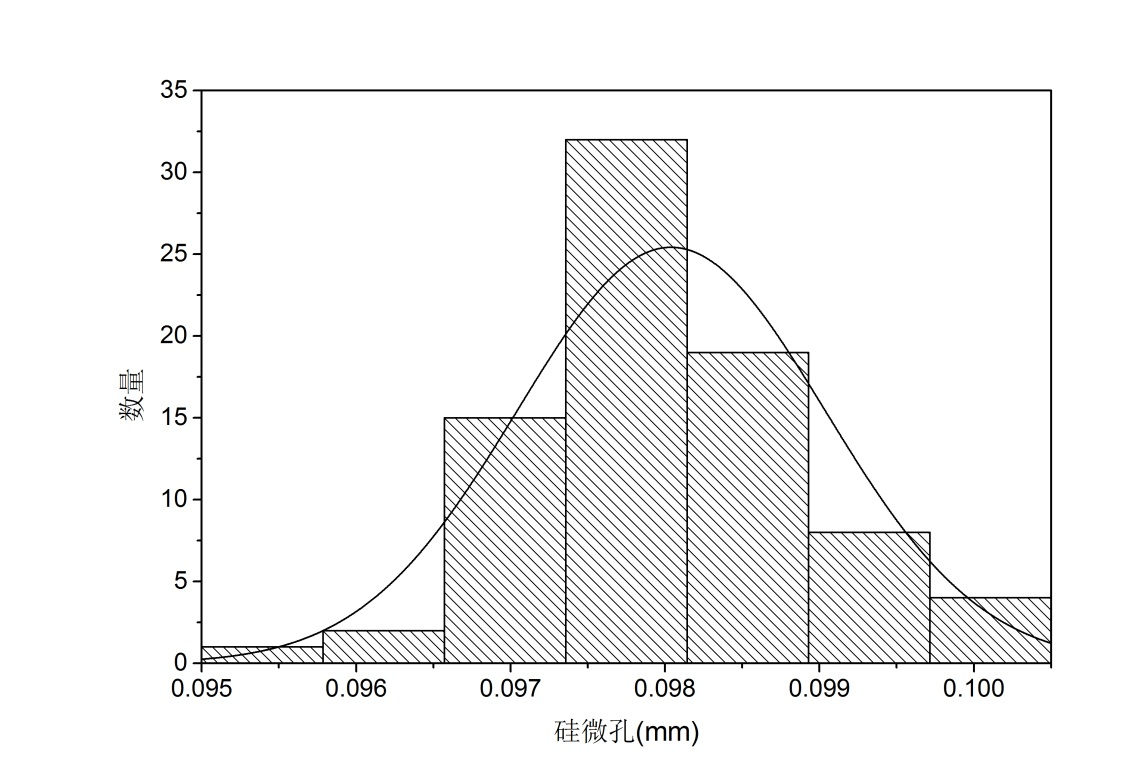
\includegraphics[width=0.72\textwidth]{assets/word-figure-3-1.jpeg}
  \caption{9×9 阵列硅微孔直径统计分布图}
  \label{fig:distribution}
\end{figure}

多幅相关图像可以组合为一幅分图，并以（a）、（b）、（c）等标出，
便于在正文中分别讨论和相互比较。

% 组合图：两个 minipage 分别承载一个分图。
\begin{figure}[htbp]
  \centering
  \begin{minipage}[t]{0.46\textwidth}
    \centering
    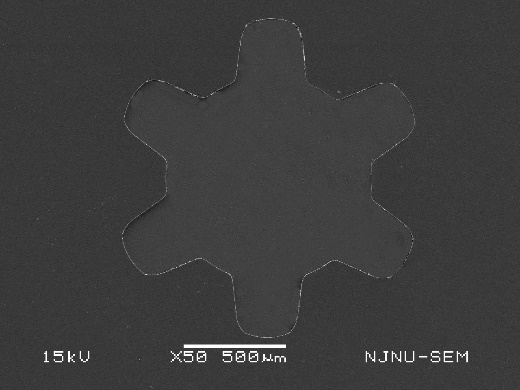
\includegraphics[width=\linewidth]{assets/word-figure-3-2a.jpeg}\\
    （a）单联硅齿轮
  \end{minipage}\hfill
  \begin{minipage}[t]{0.46\textwidth}
    \centering
    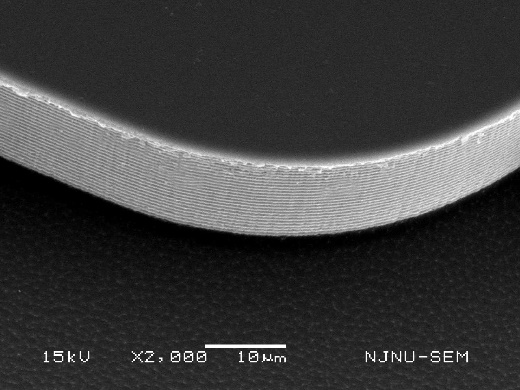
\includegraphics[width=\linewidth]{assets/word-figure-3-2b.jpeg}\\
    （b）硅齿轮局部
  \end{minipage}
  \caption{ICP 刻蚀的硅微齿轮模具 SEM 照片}
  \label{fig:sem}
\end{figure}

\subsection{表}

表格适合呈现具有共同字段、便于横向比较的数据。表头应准确概括
各列含义，数值精度和计量单位应保持一致。

% 表格：caption 和 label 写在表体之前。
\begin{table}[htbp]
  \centering
  \caption{单个硅齿轮（$z=6$）测量尺寸}
  \label{tab:gear}
  \begin{swuttable}
    \begin{tabular}{ccc}
      \toprule
      齿顶圆直径 $d_a$/mm & 齿根圆直径 $d_f$/mm
        & 同轴度误差/mm \\
      \midrule
      1.5530 & 0.9979 & 0.0129 \\
      1.5465 & 1.0003 & 0.0042 \\
      1.5571 & 0.9985 & 0.0045 \\
      1.5471 & 1.0000 & 0.0045 \\
      1.5539 & 0.9987 & 0.0098 \\
      1.5472 & 1.0004 & 0.0052 \\
      \bottomrule
    \end{tabular}
  \end{swuttable}
\end{table}

\begin{table}[htbp]
  \centering
  \caption{产品统计表}
  \label{tab:statistics}
  \begin{swuttable}
    \begin{tabular}{lrrrr}
      \toprule
      产品 & 产量 & 销量 & 产值 & 比重 \\
      \midrule
      手机   & 11000 & 10000 & 500  & 50\% \\
      电视机 &  5500 &  5000 & 220  & 22\% \\
      计算机 &  1100 &  1000 & 280  & 28\% \\
      \midrule
      合计   & 17600 & 16000 & 1000 & 100\% \\
      \bottomrule
    \end{tabular}
  \end{swuttable}
\end{table}

\section{伪代码和程序代码}

程序代码可用于说明研究中的核心算法、数据处理流程或关键实现。
以下代码给出了一个简短的控制台程序示例。

% 代码块会在空间不足时整体换页，并保持与后文的源文件顺序。
\begin{lstlisting}[language={[Sharp]C}]
using System;

namespace ConsoleApp1
{
    class Program
    {
        static void Main(string[] args)
        {
            Console.WriteLine("Hello World!");
        }
    }
}
\end{lstlisting}

% 第五章示例：说明讨论部分及论文整体组织的写作方法。
\chapter{讨论与论文组织}

\section{研究结果的解释}

讨论部分应围绕研究目标解释结果，而不是再次重复数据。作者需要分析
结果形成的原因、内在机制和适用条件，并说明结果是否支持最初提出的
研究问题或假设。对于不符合预期的结果，也应如实报告并从样本、测量、
方法假设和外部环境等方面分析可能原因。

\section{与已有研究或实践的比较}

应将主要发现与相关文献、行业标准或已有方案进行比较，说明一致之处、
差异之处及可能原因。比较对象必须具有可比性，不能忽略研究对象、
数据口径、实验条件和评价指标的差异。引用文献是为论证提供依据，
而不是用文献数量代替分析\cite{kanamori1998shaking,zhu1996fluid}。

\section{研究贡献与局限}

研究贡献应从实际完成的工作和证据出发，可以体现在新的研究对象、
数据资料、分析视角、方法改进、系统实现或应用验证等方面。贡献表述
需要与摘要和总结一致，并明确哪些成果由作者本人完成。

任何研究都受到样本、时间、数据质量、实验条件和方法假设等限制。
主动说明局限不会削弱论文价值，反而有助于读者正确理解结论边界。
局限之后可提出具体的改进方向，但不应把本应完成而未完成的核心工作
简单留作展望。

\section{论文整体组织与证据链}

\subsection{标题和章节关系}

各级标题应简明扼要，准确概括所辖内容。相邻章节之间要有清楚的逻辑
过渡，避免同一内容在多章重复出现。绪论提出的问题、研究方法、结果、
讨论和总结应形成完整证据链，最终结论必须能够在前文找到依据。

\subsection{图表、公式和正文引用}

图表与公式应先在正文中提及，再给出具体内容。例如，本示例中的
图~\ref{fig:distribution}、表~\ref{tab:gear} 和式~\eqref{eq:fourier}
均在相关段落中得到解释。修改章节或移动内容后，编号和目录应统一
更新，避免出现正文所述编号与实际对象不一致的情况。

\subsection{目录与全文复核}

目录是论文结构的集中呈现，通常列到三级标题，并应与正文标题完全
一致。定稿前应从头到尾检查题目、摘要、目录、图表清单、正文、
参考文献、致谢和附录，重点核对术语、符号、单位、编号、引用和结论
是否前后一致。

\section{学术诚信与资料留存}

使用他人的观点、文字、数据、图片、程序或方法时，应按照规范明确
标注来源。实验记录、调查问卷、数据处理过程、程序版本和重要中间
结果应妥善保存，以便指导教师审阅和后续复核。不得伪造、篡改数据，
也不得通过改写措辞掩盖未经标注的复制使用。

% 第五章示例：总结主要成果并提出后续研究方向。
\chapter{总结与展望}

\section{总结}

最后一章应着重总结毕业设计（论文）的创新点、新见解和主要研究
成果。总结是对论文主要工作、结果和论点的提炼与概括，应准确、
简明、完整且有条理，使读者能够全面了解论文的研究意义、目的和
工作内容。

总结应严格区分作者本人取得的成果与指导教师及其他研究者的成果。
评价研究工作时必须实事求是；除非有充分证据，不宜使用“首次”、
“领先”或“填补空白”等绝对化表述。

\section{展望}

展望或建议应建立在已完成工作和现有结论的基础上，对相关技术或研究
领域未来的发展方向作出合理预测，并评价研究成果的应用前景和社会
影响，为后续研究提供可借鉴的思路。


% ============================================================================
% 5. 后置部分
% ============================================================================
\backmatter

% 示例中列出数据库内全部文献；正式论文可删除 \nocite{*}，
% 仅保留正文中通过 \cite 命令实际引用的条目。
\nocite{*}
\printbibliography[heading=bibliography,title={参考文献}]

% 致谢内容请在正式提交前替换。
\begin{acknowledgements}
致谢宜以简短的文字对课题研究与论文撰写过程中曾直接给予帮助的
人员，如指导教师、答疑教师及其他人员，表达自己的谢意。致谢不仅
是一种礼貌，也是对他人劳动的尊重，是治学者应当遵循的学术规范，
内容一般限一页。正式提交前，请将本段替换为作者本人的真实致谢内容。
\end{acknowledgements}

% 附录为可选部分；不需要附录时，可删除从 \appendix 到对应内容。
\appendix
\chapter{系统主要算法代码清单}

此部分不是必需项。对于一些不宜放在正文中的重要支撑或参考材料，
可编入附录，附录一般与论文全文装订在一起，并与正文连续编排页码。

附录可包括重要的原始数据记录、详细数学推导过程、程序代码及其说明
注释、复杂图表、设计图纸、工艺过程卡、调查问卷，以及本科期间发表
的与毕业设计（论文）相关的论文、技术成果或发明专利等。

如有多个附录，应依次使用大写字母 A、B、C 等编号，每个附录均另页
开始；只有一个附录时也应编号为附录 A，并设置明确的附录标题。

\end{document}
